%!TEX root = ../main.tex

\section{Implementation} \label{sec:implementation}
For implementing our genetic algorithm we have used an open-source clone of pac-man made in C\# by Brian Bender~\footnote{Pac-man C\# implementation:~\url{https://www.planet-source-code.com/vb/scripts/ShowCode.asp?txtCodeId=5669&lngWId=10}}.

\subsection{Modes}
The open-source version of pac-man, which we are using as a base for the implementation, did not include ghost behaviour modes (see~\ref{ssec:design_modes}).
The ghosts do not actively chase pacman or scatter to individual corners as in the original pac-man.
They move by randomly selecting a point from a list of moveable points.

\begin{lstlisting}[caption=random movement, label=lst:imp1]
if (currentMode == Cycle.MonsterMode.IsRandom) {
	ArrayList pts = GetNextPossibleCoordinates(_direction, _currentLocation);
	int iSelected = _rnd.Next(1, pts.Count + 1);
	Point SelectedPoint = (Point)pts[iSelected - 1];

	if (_currentLocation.Y < SelectedPoint.Y)
	_direction = CharacterDirection.Down;
	else if (_currentLocation.X < SelectedPoint.X)
	_direction = CharacterDirection.Right;
	else if (_currentLocation.X > SelectedPoint.X)
	_direction = CharacterDirection.Left;
	else if (_currentLocation.Y > SelectedPoint.Y)
	_direction = CharacterDirection.Up;

	MoveToEndPoint(_direction, GetDestinationCoordinate(_direction, _currentLocation));
}
\end{lstlisting}

As inspiration for movement patterns (aka modes) we referred to how the original pac-man moved the ghosts~\autocite{Mateas2003}.
These would become the ghost \emph{modes}.
The important thing was not to mimic pac-man exactly but rather to have different parameters for the ghosts behaviours to cycle through in the GA.

Although no modes or pathfinding was present in the source code, it did include methods for movement of the ghosts, \texttt{Move()}, and collision detection, \texttt{CanMove()}.
We used these pre-existing methods to do the actual movement of the ghosts, but in order to do \emph{chase} and \emph{scatter} we needed a pathfinding system.

\subsubsection*{pathfinding + neighbors}
Originally, an A* search algorithm was implemented (See appendix~\ref{sec:astar}) as a pathfinder, but it proved a hog on the system resources, so a much simpler method was created, inspired by the pathfinding of the original pac-man (See Analysis~\ref{ssub:pathfinding}).

The way pathfinding was done, four \emph{neighbors} were created one point left, right, below and above the ghost’s current location.

\begin{lstlisting}[caption=Neighbor class, label=lst:neighbor]
public class Neighbors
{
	int x;
	int y;
	private double distance;

	public int X
	{
		get { return x; }
		set { x = value; }
	}

	public int Y
	{
		get { return y; }
		set { y = value; }
	}

	public double Distance
	{
		get { return distance; }
		set { distance = value; }
	}
}
\end{lstlisting}

\begin{lstlisting}[caption=Instantiate neighbors, label=lst:instantiateneighbors]
//Create List<> to contain each neighbor of the ghost in question.
List<Neighbors> neighbors = new List<Neighbors>();

//Create four neighbors right, left, above and below the ghosts current location.
Neighbors rightNeighbor = new Neighbors() { X = currentLocation.X + 1, Y = currentLocation.Y };
Neighbors leftNeighbor = new Neighbors() { X = currentLocation.X - 1, Y = currentLocation.Y };
Neighbors aboveNeighbor = new Neighbors() { X = currentLocation.X, Y = currentLocation.Y + 1 };
Neighbors belowNeighbor = new Neighbors() { X = currentLocation.X, Y = currentLocation.Y - 1 };
\end{lstlisting}

Then a check was done to see if the ghost could move to the individual neighbor’s location.

\begin{lstlisting}[caption=canMove check, label=lst:canMove]
//If the ghost can move to the location of the neighbor and the ghosts current direction is not the opposite
//of the direction of the neighbor, add that neighbor to the neighbors List<>.
if (board.CanMove(new Point(rightNeighbor.X, rightNeighbor.Y)) && direction != CharacterDirection.Left)
neighbors.Add(rightNeighbor);
if (board.CanMove(new Point(leftNeighbor.X, leftNeighbor.Y)) && direction != CharacterDirection.Right)
neighbors.Add(leftNeighbor);
if (board.CanMove(new Point(aboveNeighbor.X, aboveNeighbor.Y)) && direction != CharacterDirection.Down)
neighbors.Add(aboveNeighbor);
if (board.CanMove(new Point(belowNeighbor.X, belowNeighbor.Y)) && direction != CharacterDirection.Up)
neighbors.Add(belowNeighbor);
\end{lstlisting}

If the neighbor’s location was moveable, the distance of that neighbor’s location and the location of pac-man, was calculated.

\begin{lstlisting}[caption=calculate distances,label=lst:distance]
//Create List<> to contain the distances of each neighbor to pac-man.
List<double> distances = new List<double>();

//Calculate distance from neighbors to pac-man.
foreach (Neighbors n in neighbors)
{
	n.Distance = Distance(new Point(n.X, n.Y), pacmanLocation);
	if (!distances.Contains(n.Distance))
	distances.Add(n.Distance);
}
\end{lstlisting}

\begin{lstlisting}[caption=Distance method,label=lst:distanceMethod]
//Calculate distance between passed Points. In this case the distance between each ghost neighbor and pac-man.
public double Distance(Point from, Point to)
{
	double a = from.X - to.X;
	double b = from.Y - to.Y;
	double distance = Math.Sqrt(a * a + b * b);
	return distance;
}
\end{lstlisting}

The neighbor with the shortest distance to pac-man would then determine the ghost’s next point to move to.

\begin{lstlisting}[caption=select point,label=lst:selectPoint]
//The neighbor (contained in neighbors List) which has the same distance as the first item
//in sorted List distances (shortest distance from pac-man), decides the point (relative to the ghost) which the ghost has to move to.
if (neighbors.Contains(rightNeighbor) && rightNeighbor.Distance == distances[0])
go = new Point(1, 0);

else if (neighbors.Contains(leftNeighbor) && leftNeighbor.Distance == distances[0])
go = new Point(-1, 0);

else if (neighbors.Contains(aboveNeighbor) && aboveNeighbor.Distance == distances[0])
go = new Point(0, 1);

else if (neighbors.Contains(belowNeighbor) && belowNeighbor.Distance == distances[0])
go = new Point(0, -1);

//return the point closest to pac-man which the ghost can move to.
return go;

\end{lstlisting}

The ghosts only check for a new move location and direction at every intersection in the game level, and so a method was created to generate a lists of the location of every intersection.

\begin{lstlisting}[caption=generate intersections,label=intersections]
//Generate HashSet<> which contains every intersection in the current level.
public void GenerateIntersections()
{
	intersections = new HashSet<Point>();

	intersections.Add(new Point(23, 26));
	intersections.Add(new Point(199, 26));
	intersections.Add(new Point(246, 26));
	intersections.Add(new Point(422, 26));
	intersections.Add(new Point(23, 97));
	intersections.Add(new Point(422, 97));
	intersections.Add(new Point(23, 150));
	intersections.Add(new Point(103, 150));
	intersections.Add(new Point(103, 256));
	intersections.Add(new Point(342, 256));
	intersections.Add(new Point(103, 97));
	intersections.Add(new Point(342, 97));

\end{lstlisting}

A foreach loop would check if the ghost’s location was equal to an intersection, and if so, pass the returned point from the Pathfinder method as the selected point to move towards.

\begin{lstlisting}[caption=pathfinder call,label=lst:pathfinderCall]
if (Pathfinder.Intersections.Contains(_currentLocation))
{
	go = pathfinder.ClosestNeighbor(_currentLocation, pacmanCurrentLocation, _board, _direction);
}

SelectedPoint = new Point(_currentLocation.X + go.X, _currentLocation.Y + go.Y);

if (_currentLocation.Y < SelectedPoint.Y)
_direction = CharacterDirection.Down;
else if (_currentLocation.X < SelectedPoint.X)
_direction = CharacterDirection.Right;
else if (_currentLocation.X > SelectedPoint.X)
_direction = CharacterDirection.Left;
else if (_currentLocation.Y > SelectedPoint.Y)
_direction = CharacterDirection.Up;

MoveToEndPoint(_direction, GetDestinationCoordinate(_direction, _currentLocation));
\end{lstlisting}

\subsection{Modes and Cycle}\label{ssec:modesCycle}
The \emph{GhostCharacter} class contains a Method called \emph{MoveMonster()}. What this method does is it moves the monster one time per frame, depending on what current mode is set for that ghost. The mode is controlled by a private variable called \emph{currentMode}. This is of the type \emph{MonsterMode} which is a custom enumerator, which is defined by the \emph{Cycle} class as described later. In the original source code, this method was used to move the ghosts randomly, and to animate them as well.

In order to make the ghosts move according to their \emph{MonsterMode}, we expanded the method with if statements as such:
\begin{lstlisting}
if (currentMode == Cycle.MonsterMode.IsRandom) {
\end{lstlisting}

This will instead make the ghost move according to their \emph{MonsterMode}, as described in the previous chapter.

The same is true of the MonsterModes \emph{IsChasing} and \emph{IsScattering}.

\subsubsection*{The Cycle}
Now we know that in order to make our ghosts move independently, we simply need to change their current MonsterMode. The idea of the cycle is that each ghost will independently have their MonsterMode changed, according to whatever parameters we (or the Genetic Algorithm) give them. This is where the custom made Cycle class comes in handy.

\begin{lstlisting}[caption=Cycle class and its constructor,label=lst:cycle]
using System;
using System.Collections.Generic;
using System.Linq;
using System.Text;

namespace Chomp
{
	[Serializable]
	public class Cycle
	{
		public enum MonsterMode
		{
			IsRandom = 0,
			IsChasing = 1,
			IsScattering = 2,
			IsFleeing = 3
		}
		public Cycle(MonsterMode mode, double cyclevalue)
		{
			Mode = mode;
			CycleValue = cyclevalue;
		}

		public MonsterMode Mode { set; get; }
		public double CycleValue { set; get; }

	}
}
\end{lstlisting}

The \emph{Cycle} class is the basis we use to switch between the different ghost modes. In the \emph{GhostCharacter} class, we have a member which is a  \emph{List<T>} of 3 \emph{Cycles}, called \emph{cycle}.
It is essential that it is a List, due to the fact that we have three different modes to cycle between. Each Cycle in the list contains a Mode and a CycleValue. The Mode is the previously described MonsterMode, and the CycleValue is the duration of each Mode. The CycleValue can also be translated into percentage, so each List’s Cycles have a total CycleValue sum of 100.

The usage of this system is as follows:
\begin{lstlisting}[caption=Snippet of GameBoard.cs and Cycle instantiation,label=lst:cycleInst]
initialCycle = new Cycle(Cycle.MonsterMode.IsChasing, 33.3);
initialCycleList = new List<Cycle>();
initialCycleList.Add(initialCycle);
initialCycle = new Cycle(Cycle.MonsterMode.IsRandom, 33.3);
initialCycleList.Add(initialCycle);
initialCycle = new Cycle(Cycle.MonsterMode.IsScattering, 33.3);
initialCycleList.Add(initialCycle);
\end{lstlisting}

We create 3 cycles each with a unique mode, and a total sum of 100, and add them each to our List. This List can then be applied to any ghost and it will follow the respective cycle, which in turn also is the way we apply it for the initial playthrough for the prototype, where initial playthrough in this case means the first time a test person plays the game.

This all comes together in the GameBoard class, where we call the method \emph{UpdateCycle()} on each frame for each ghost.

\begin{lstlisting}[caption=Snippet of GameBoard.cs showing the system to Cycle between modes for ghosts, label=lst:cycleModes]
public void UpdateCycle(GhostCharacter g)
{

	if (g.CycleUpdaterInternal >= 50 && g.CurrentInvinsibility != CharacterInvincibility.Vulnerable)
	{
		if (g.CurrentModeValue == 0)
		{
			if (g.CurrentCycle[0].CycleValue * 10 <= cycleUpdaterBigFrame)
			{
				Console.WriteLine("Switching to 1 from " + g.CurrentMode);
				g.CurrentMode = g.CurrentCycle[1].Mode;
				g.CurrentModeValue = 1;
			}
		}
		else if (g.CurrentModeValue == 1)
		{
			double t = 10 * g.CurrentCycle[0].CycleValue;
			if (t + g.CurrentCycle[1].CycleValue * 10 <= cycleUpdaterBigFrame)
			{
				Console.WriteLine("Switching to 1 from " + g.CurrentMode);
				g.CurrentMode = g.CurrentCycle[2].Mode;
				g.CurrentModeValue = 2;
			}
		}
		else if (g.CurrentModeValue == 2)
		{
			if (cycleUpdaterBigFrame >= 1000)
			{
				Console.WriteLine("Switching to 0 from" + g.CurrentMode);
				g.CurrentMode = g.CurrentCycle[0].Mode;
				g.CurrentModeValue = 0;
				cycleUpdaterBigFrame = 0;
			}

		}
		g.CycleUpdaterInternal = 0;
	}
	g.CycleUpdaterInternal++;
}
\end{lstlisting}

The method takes a GhostCharacter as input. The \emph{cycleUpdaterBigFrame} is an integer that runs from 0 to 1000, counting each frame. Depending on this, and a couple of other checks to ensure that the cycle is running accurately, it will change the MonsterMode of the individual ghost and reset the integer to reset the cycle. Using 1000 and multiplying by 10 is how we get the \emph{CycleValue} double to represent percentage.

the \emph{CycleUpdaterInternal} integer is in place to avoid running through the check on every frame, but only checks once per 50 frames for each ghost, which corresponds to about 1 second per check when playing the prototype in real time, since it is timed to run at one frame per 20 milliseconds during normal play.

This concludes how we control the behaviour for each ghost individually, how the different modes work, and how we switch between the modes.

\subsection{Flow}
\subsubsection*{Initial playthrough}
Before we move into the Genetic Algorithm part of the prototype, we will go over the flow of how the prototype progresses.

The Pac-Man clone is made in Windows Forms, so the initial startup of the application simply generates the form and it’s parameters, which can all be found in the frmScreen class. We’ve added additional variables and modified some values from the original to fit our needs better, such as changing the lives to 1 instead of 3, and adding a \emph{List<CharacterDirection>} member to record the player’s movement.

\begin{lstlisting}[caption=Snippet of frmScreen.cs taken from the key event handler, label=lst:keyEvent]
else if (e.KeyCode == Keys.F1)
{
	if (_board.Player2.GameOver)
	{
		GeneticStuff = new GA();
		GeneticStuff.InitializeGA();
		recordDirection.Clear();
		_board.CurrentPlayer.Score = 0;
		recording = true;
		recordTicker = 0;
		this.tmrMove.Interval = 20;
		this.microTimer.Enabled = false;

		StartGame(1);
\end{lstlisting}

The gameplay is started by pressing F1 on the initial splash screen.
Controlled by the key event handler frmScreen\_Keydown, this will call StartGame(1), instantiate the GA
 class for later use, as well as adjusting settings for playing the game and not simulating.

In StartGame(),  the GameBoard and characters (Pac-Man and ghosts) are instantiated. The last thing that happens in this method is the timer being started. The timer is of the type Windows.Forms.Timer and is set to run at an interval of 20 milliseconds. This begins the game.

The game advances by using the tmrMove\_Tick() event method, which is triggered at the interval of the Windows.Forms.Timer.

\begin{lstlisting}[caption=Snippet of frmScreen. A method called at each timer interval, label=lst:timerInterval]
private void tmrMove_Tick(object sender, System.EventArgs e)
{
	if (powerMode)
	{
		if (powerTicker > 90)
		{
			tmrPowerMode_Tick();
		}

		powerTicker++;

	}
	if (recording)
	{
		recordDirection.Add(_board.PacMan.AttemptedDirection);
		recordTicker++;
		_board.MoveCharacters();
		picGameBoard.Invalidate();
	}

	else if (!recording && normalPlayback)
	{
		if (recordTicker > playbackTicker)
		{
			_board.PacMan.AttemptedDirection = recordDirection[playbackTicker];
			playbackTicker++;
		}
		_board.MoveCharacters();
		picGameBoard.Invalidate();
	}
}

\end{lstlisting}

This method controls a few different things. As we need to run the game at a much faster speed when simulating, it was not appropriate to use a timer solution for triggering the state of the ghosts’ vulnerability, so this has been changed to be controlled by counting frames. If the boolean recording is true, it will record the players direction per frame and add it to the previously mentioned list. It will then call the MoveCharacters() method of the GameBoard class.

\begin{lstlisting}[caption=Snippet of GameBoard.cs. Method used to move and check collision for each character.,label=lst:collision]
public void MoveCharacters()
{
	UpdateCycle(_ghostRed);
	UpdateCycle(_ghostBlue);
	UpdateCycle(_ghostPink);
	UpdateCycle(_ghostYellow);
	_pacMan.Move();
	_ghostRed.MoveMonster();
	_ghostPink.MoveMonster();
	_ghostBlue.MoveMonster();
	_ghostYellow.MoveMonster();
	cycleUpdaterBigFrame++;

	GameCharacter g = PlayerCollided(_pacMan, _ghostRed, _ghostPink, _ghostBlue, _ghostYellow);

	if ( g != null)
	{
		Console.WriteLine(g);
		if (g.CurrentInvinsibility == CharacterInvincibility.Vulnerable)
		{
			g.Visible = false;
			_pacMan.Visible = false;
			_currentPlayer.Score += _currentEatScore;
			UpdateScore();
			if (frmScreen.recording)
			{
				_picGameBoard.Refresh();
				PaintEatScore(new Point(g.CurrentLocation.X - 15, g.CurrentLocation.Y - 10), Graphics.FromHwnd(_picGameBoard.Handle));
			}
			_currentEatScore *= 2;
			_pacMan.Visible = true;
			ResetMonster(g);
			if (frmScreen.recording)
			_picGameBoard.Refresh();

\end{lstlisting}

We already know what UpdateCycle() and MoveMonster() has do, as it is explained in~\ref{ssec:modesCycle} Move() is responsible for moving pacman depending on his current CharacterDirection.

The rest of this method is responsible for the collision detection. If Pac-Man and any of the ghosts collide with each other, the player’s turn will either end, or he will eat the ghost he collided with, depending on the ghost’s vulnerability status.

The following flow chart (figure~\ref{fig:imp1}) helps visualize the process of the initial playthrough:

\begin{figure}[!htbp]
	\centering
	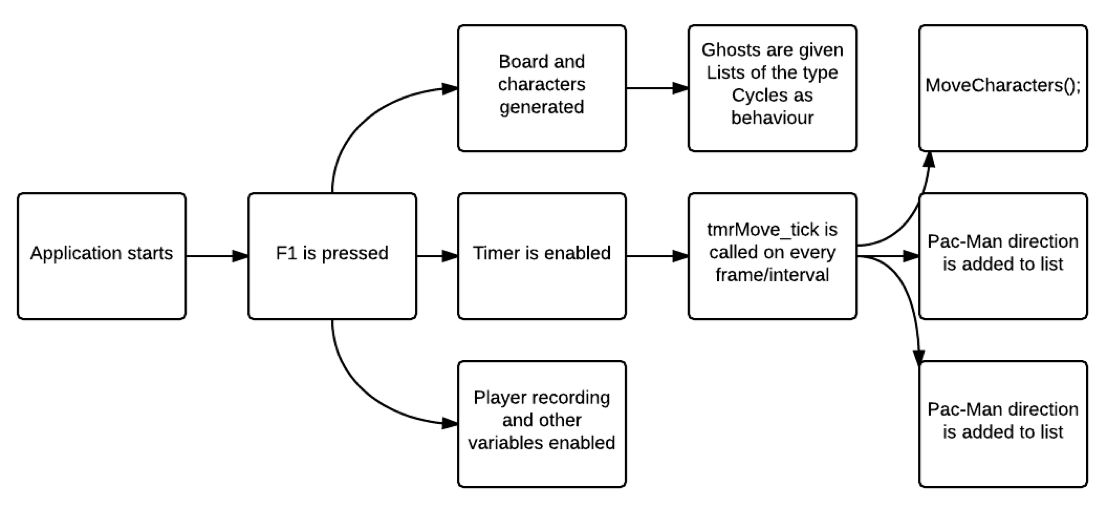
\includegraphics[width=0.95\textwidth]{imp_1.png}
	\caption{Flow of normal gameplay}
	\label{fig:imp1}
\end{figure}

\subsubsection*{Simulation}
The flow for simulations are fairly similar to initial playthrough.

\subsubsection*{Timer while simulating}
Instead of the timer being set to 20 ms, we gave it a value of 1 ms instead and tried running simulations with this. It was later discovered that the Windows.Forms.Timer has internal limitations, that prevent it from running faster than around 14 ms. This was very clear as simulations were not running much faster than when playing the game at normal spear.

This led us to trying to find a different way than using a Forms timer, and the first solution we tried implementing was running a continuous while loop, that would only end if the player died or won the game.

However, this also caused some problems. During testing with this implementation, we discovered that collision detection was nowhere near fast enough to keep up with the while loop, as the while loop would move the characters as fast as the CPU can handle, not allowing the collision detection of the game to react in time.

We attempted many different solutions to counteract this problem, such as creating async functions that would wait for each other, delaying the while loop substantially by making it process fake data, and trying to improve the Pac-Man clone’s collision detection.

Ultimately, we ended up not being able to use a while loop, and instead we came up with the solution of using the System.Diagnostics.Stopwatch as a timer instead. This Stopwatch class is not intended to be used as a timer, but we found a wrapper which allows it to be, by creating a subclass that uses the Stopwatch, allowing us to instantiate an extremely fast timer~\footnote{\url{http://www.codeproject.com/Articles/98346/Microsecond-and-Millisecond-NET-Timer}}. Since we did not need precision, but rather speed, it was not a problem if the timer was not accurate to the nanosecond.

Simulating with this timer had good results, as the game’s logic and collision detection was able to keep up. Testing at 0.5 ms sometimes lead to graphical glitches, as the GameBoard is refreshed on every frame. When this happens the game is unable to recover, and collision is broken for the rest of the time the application is run. The timer ended up being set to about 1.8 ms, which allowed us to have reasonably fast simulations and also keep collision detection.

\subsubsection*{Playback}
As mentioned before, the player’s CharacterDirection is recorded every frame, which allows us to run through this recording, and play it back once per frame accordingly. Since there are no physics involved, the playback will always match the input of the player.

\begin{lstlisting}[caption=Snippet of frmScreen.cs. High resolution timer event method, label=lst:timer]
private void moveTick_while(object sender, MicroTimerEventArgs timerEventArgs)
{
	if (powerMode)
	{
		if (powerTicker > 90)
		{
			tmrPowerMode_Tick();
		}
		powerTicker++;
	}
	if (recordTicker > playbackTicker)
	{
		_board.PacMan.AttemptedDirection = recordDirection[playbackTicker];
		playbackTicker++;
		_board.MoveCharacters();
		picGameBoard.Invalidate();
	}
	if (recordTicker <= playbackTicker)
	{
		_board.MoveCharacters();
		picGameBoard.Invalidate();
	}
}
\end{lstlisting}

On each frame, we run a check on whether or not the playback frame is smaller than the recorded frame, and if it is, we will set Pac-Man’s direction to the matching direction on the frame it was recorded. If however there is nothing more to play back, the game will still as before, but Pac-Man will no longer move. A case for this could be where the player died very quickly, but on the simulation the ghosts will have a different behaviour, making them reach Pac-Man at a later time.

\subsection{Genetic Algorithm}
\subsubsection*{Framework}
For implementing a Genetic Algorithm to handle our calculations, we have chosen to use the Genetic Algorithm Framework (GAF) for .NET 4 and 4.5~\footnote{\url{http://aiframeworks.net/}}.
The framework is easily available through the NuGet package manager, and can be installed using Visual Studio’s console.

As inspiration for our own implementation, we took a close look at their example for “The Travelling Salesman”, and how they have gone about solving it~\footnote{\url{http://aiframeworks.net/blog/gaf-part-4}}.

This framework allows us to use objects as genes, which is perfect as we can cast them into the List of Cycles that we need for each ghost. The chromosomes are supposed to be a solution for each time we run a simulation, which means the chromosome needs to be created of 4 different genes, one gene for each ghost. According to previous research (~\ref{ssub:population}, a decent sized population ranges from 20 to 100, so we have decided to go with 20 chromosomes per generation for our prototype.

\subsubsection*{Gene creation (first generation)}
As mentioned before, each ghost must have a List of Cycles in order to control their behaviour. Our initial gene creation creates completely random genes for each ghost. These are then collected and added to a single gene. Twenty of these make up our population.

\begin{lstlisting}[caption=Snippet of GA.cs. Gene creation method, label=lst:genes]
private List<Cycle> CalculateGenes()
{
	List<Cycle> gene = new List<Cycle>();

	Cycle cycle1;
	Cycle cycle2;
	Cycle cycle3;

	//Random rnd = new Random();
	int r;

	double alpha = 0, beta = 0, gamma = 0, k = 0;

	alpha = rnd.Next(0, 100);
	beta = rnd.Next(0, 100);
	gamma = rnd.Next(0, 100);

	k = (alpha + beta + gamma) / 100;

	alpha /= k;
	beta /= k;
	gamma /= k;

	List<Cycle.MonsterMode> monsterList = new List<Cycle.MonsterMode>();
	monsterList.Add(Cycle.MonsterMode.IsRandom);
	monsterList.Add(Cycle.MonsterMode.IsChasing);
	monsterList.Add(Cycle.MonsterMode.IsScattering);

	r = rnd.Next(monsterList.Count);
	cycle1 = new Cycle(monsterList[r], alpha);
	monsterList.Remove(monsterList[r]);

	r = rnd.Next(monsterList.Count);
	cycle2 = new Cycle(monsterList[r], beta);
	monsterList.Remove(monsterList[r]);
	r = rnd.Next(monsterList.Count);
	cycle3 = new Cycle(monsterList[r], gamma);
	monsterList.Remove(monsterList[r]);

	gene.Add(cycle1);
	gene.Add(cycle2);
	gene.Add(cycle3);

	return gene;
}
\end{lstlisting}

The List of Cycles is first created, then populated with random values that have a total sum of 100, and a random MonsterMode. This process is repeated 4 times for each chromosome.

\begin{lstlisting}[caption=Snippet of GA.cs. Adding genes to chromosomes, label=lst:geneChromosome]
population = new Population(20); // Amount of simulations
ghostChromosomes = new List<List<Cycle>>();
//Fill our population with chromosomes, which each contain 4 genes.
for (int p = 0; p < 10; p++)
{
	ghosts = new List<List<Cycle>>();
	ghosts = CreateGhosts();
	Chromosome chromosome = new Chromosome();
	for (int h = 0; h <= 3; h++)
	{
		chromosome.Genes.Add(new Gene(ghosts[h]));

	}
	population.Solutions.Add(chromosome);
}
\end{lstlisting}

\subsubsection*{Simulations using the Genetic Algorithm}
We create our population and fill it with the chromosomes generated by the previous method. When the game simulates, we give each ghost one of our created genes, from the list of chromosomes. This is done as such:

\begin{lstlisting}[caption=Snippet of frmScreen.cs. Key event handler starting the simulation, label=lst:keyHandler]
else if (e.KeyCode == Keys.F9)
{
	runNumber++;
	tmrBlink.Enabled = true;
	var t = GeneticStuff.FittestPerGeneration;
	_board.Blinky.CurrentCycle = (List<Cycle>)t.Genes[0].ObjectValue;
	_board.Inky.CurrentCycle = (List<Cycle>)t.Genes[1].ObjectValue;
	_board.Pinky.CurrentCycle = (List<Cycle>)t.Genes[2].ObjectValue;
	_board.Clyde.CurrentCycle = (List<Cycle>)t.Genes[3].ObjectValue;
	_board.Blinky.CurrentMode = _board.Blinky.CurrentCycle[0].Mode;
	_board.Inky.CurrentMode = _board.Inky.CurrentCycle[0].Mode;
	_board.Pinky.CurrentMode = _board.Pinky.CurrentCycle[0].Mode;
	_board.Clyde.CurrentMode = _board.Clyde.CurrentCycle[0].Mode;
	Console.WriteLine(_board.Blinky.CurrentCycle[0].Mode + " " + _board.Inky.CurrentCycle[0].Mode + " " + _board.Pinky.CurrentCycle[0].Mode + " " + _board.Clyde.CurrentCycle[0].Mode);

	recordDirection.Clear();
	_board.CurrentPlayer.Score = 0;
	recording = true;
	recordTicker = 0;
	this.tmrMove.Interval = 20;
	this.microTimer.Enabled = false;

	StartGame(1);
}
\end{lstlisting}

We cast each gene to a List of Cycles, and assign them to our ghost. We then set the mode of each ghost to be the first mode in it’s newly given List of Cycles. We then set the score to 0 and start our high resolution timer, in order to evaluate the proposed solution.

This is only for the first simulation in a generation. We have automated the process to evaluate the rest of the chromosomes in the population as well.

If Pac-Man is killed or is successful in eating all the pellets, UpdateChromosome() is called.

\begin{lstlisting}[caption=Snippet of frmScreen.cs. UpdateChromosome method to change chromosome for each simulation, label=lst:updateChromosome]
private void UpdateChromosome(int s, bool w=false)
{
	Logger previousRun = new Logger();
	previousRun.Score = s;
	previousRun.LoggedChromosome = GeneticStuff.population.Solutions[currentChromosome-1];
	Console.WriteLine(GeneticStuff.population.Solutions[currentChromosome - 1].Id);
	previousRun.WinLoss = w;
	currentRunLog.Add(previousRun);

	if (currentChromosome < GeneticStuff.population.Solutions.Count)
	{
		_board.CycleUpdaterBigFrame = 0;
		int t = currentChromosome;

		_board.Blinky.CurrentCycle = (List<Cycle>)GeneticStuff.population.Solutions[t].Genes[0].ObjectValue;
		_board.Inky.CurrentCycle = (List<Cycle>)GeneticStuff.population.Solutions[t].Genes[1].ObjectValue;
		_board.Pinky.CurrentCycle = (List<Cycle>)GeneticStuff.population.Solutions[t].Genes[2].ObjectValue;
		_board.Clyde.CurrentCycle = (List<Cycle>)GeneticStuff.population.Solutions[t].Genes[3].ObjectValue;
		_board.Blinky.CurrentMode = _board.Blinky.CurrentCycle[0].Mode;
		_board.Inky.CurrentMode = _board.Inky.CurrentCycle[0].Mode;
		_board.Pinky.CurrentMode = _board.Pinky.CurrentCycle[0].Mode;
		_board.Clyde.CurrentMode = _board.Clyde.CurrentCycle[0].Mode;
		SimulationFast();
		Console.WriteLine(currentChromosome);
		Console.WriteLine(s);

	}
\end{lstlisting}

UpdateChromosome() takes 2 arguments, an int representing the score for the simulation and a boolean representing whether or not the simulation won. For this purpose we have created another custom Class, which we use as a type to log data for each of the simulations. We store the score, the ID for the respective chromosome, as well as whether or not the player won.

We then make a check if there are more chromosomes left in the current population to run through, and if so we give the ghosts the next List of Cycles, or genes, and run the simulation again.

Once there are no more simulations, we call on the GA to evaluate the simulations and assign them a fitness score.


\begin{lstlisting}[caption=Snippet of frmScreen.cs continued. Starting the GA and evaluation, label=lst:gaEvo]
microTimer.Enabled = false;
Console.WriteLine("done simulating");
ga = new GeneticAlgorithm(GeneticStuff.population, CalculateFitness);
int c = 0;
foreach (object o in currentRunLog)
{
	//Console.WriteLine(currentRunLog[c].LoggedChromosome.Id + " " + ga.Population.Solutions[c].Id);
	c++;

}
ga.OnGenerationComplete += GeneticStuff.ga_OnGenerationComplete;
ga.OnRunComplete += GeneticStuff.ga_OnRunComplete;
ga.Operators.Add(GeneticStuff.elite);
ga.Operators.Add(GeneticStuff.crossover);
ga.Operators.Add(GeneticStuff.mutate);
if (runNumber > 0)
{
	foreach (Chromosome p in ga.Population.Solutions)
	{
		p.Evaluate(CalculateFitness);
	}
}
ga.Run(Terminate);
\end{lstlisting}

We instantiate the GeneticAlgorithm(GA) type which is defined by the GAF. This takes a population and a method for calculating fitness as arguments.
We then subscribe to our event handlers, and add our operators to the Genetic Algorithm.

We then tell the algorithm to start, with Terminate as the method for when it should stop. In our case, the Terminate is set to stop after two generations, because we can only give it the score of each simulation for one generation at a time.

However, allowing it to run for two generations lets the GA first evaluate the score for each simulation, and then create a new population based on the results of this. This has the backwards effect of giving all the chromosomes in the second generation a fitness value of 1, as our fitness function will always return 0 as score.

In order to solve this problem, we implement a check to check what generation we are currently evaluating. If this is above 0, then it will force a re-evaluation of all the chromosomes in a population. As we store the chromosome IDs in the List of Loggers, we can always match a simulation and chromosome to each other, which makes this re-evaluation possible.

\subsubsection*{Fitness Function}
Our fitness function works quite simply by checking what the final score was for a simulation. The chromosome is given a fitness level based on this.

\begin{lstlisting}[caption=snippet of frmScreen.cs. Methods to calculate fitness for each chromosome., label=lst:fitness]
public double CalculateFitness(Chromosome chromosome)
{
	double min = 3000;
	double score = 1-(GetScoreFromRun(chromosome)/ min);
	return score;
}
public int GetScoreFromRun(Chromosome chromosome)
{
	int c = 0;
	int q = 0;
	Console.WriteLine(chromosome.Id);
	if (chromosome != null)
	{
		foreach (object o in currentRunLog)
		{
			if (chromosome.Fitness == 1 && currentRunLog[c].LoggedChromosome.Id == chromosome.Id)
			{
				Console.WriteLine("something went wrong");
			}
			if (currentRunLog[c].LoggedChromosome.Id == chromosome.Id)
			{
				q = currentRunLog[c].Score;
				Console.WriteLine(currentRunLog[c].LoggedChromosome.Id + " " + chromosome.Id);

			}
			c++;
		}
	}
	return q;
}
\end{lstlisting}

In the first edition of the prototype, the worst case scenario for the ghosts are that Pac-Man gets a score of 3000. This will later be revised through pre-testing, finding a more optimal value to evaluate against.
For each chromosome that runs through the CalculateFitness() method, GetScoreFromRun() is also called. In this method, we match the chromosome given as argument against a logged chromosome, using the unique ID string that GAF gives it. This also means that if the chromosome can’t be matched to a logged simulation, it will return a score of 0, giving the chromosome the best possible evaluation. This is why we need to re-evaluate once the simulations have actually been run, as mentioned before.

\subsubsection*{Logger class}
\begin{lstlisting}[caption=Logger class and its constructor.,label=lst:logger]
namespace Chomp
{
	[Serializable]
	public class Logger
	{
		public Logger()
		{
			WinLoss = false;
		}

		public int Score { set; get; }
		public bool WinLoss { set; get; }
		public Chromosome LoggedChromosome { set; get; }
	}
}
\end{lstlisting}

For each simulation we store a Logger object in a List. This is simply to keep track of the runs and to be sure that the evaluated chromosome matches the chromosome for that particular simulation.

As we store a Chromosome object in each Logger, we can directly match it using the unique ID-string given by the GAF.

\subsubsection*{Genetic Algorithm Operators}
Some operators are pre-made and come as part of the GAF. Although it is a possibility to create your own operators, our research indicates that the operators included will suit our needs (see \ref{ssub:population}).The operators that we have in use are Elite~\footnote{\url{http://aiframeworks.net/microsites/gaf/html/9a476085-c561-dc6d-f30e-69e720795e1c.htm}}, SwapMutate~\footnote{\url{http://aiframeworks.net/microsites/gaf/html/7677aa9e-d365-3e26-cf64-376f994b1f45.htm}} and CrossOver~\footnote{\url{http://aiframeworks.net/microsites/gaf/html/49d4e899-e9a0-473e-815a-e2b3a35d2465.htm}}

The parameters chosen for each operator are inspired by “The Travelling Salesman” example, and these values correspond with our research for each operator (see \ref{ssub:population}).


We have created a class diagram which shows the inheritance and interfacing between all the classes, to help give a better understanding of how the prototype is working. The class diagram can also be seen in expanded form in the appendix, where we have all the members of each class visible.

\begin{figure}[!htbp]
	\centering
	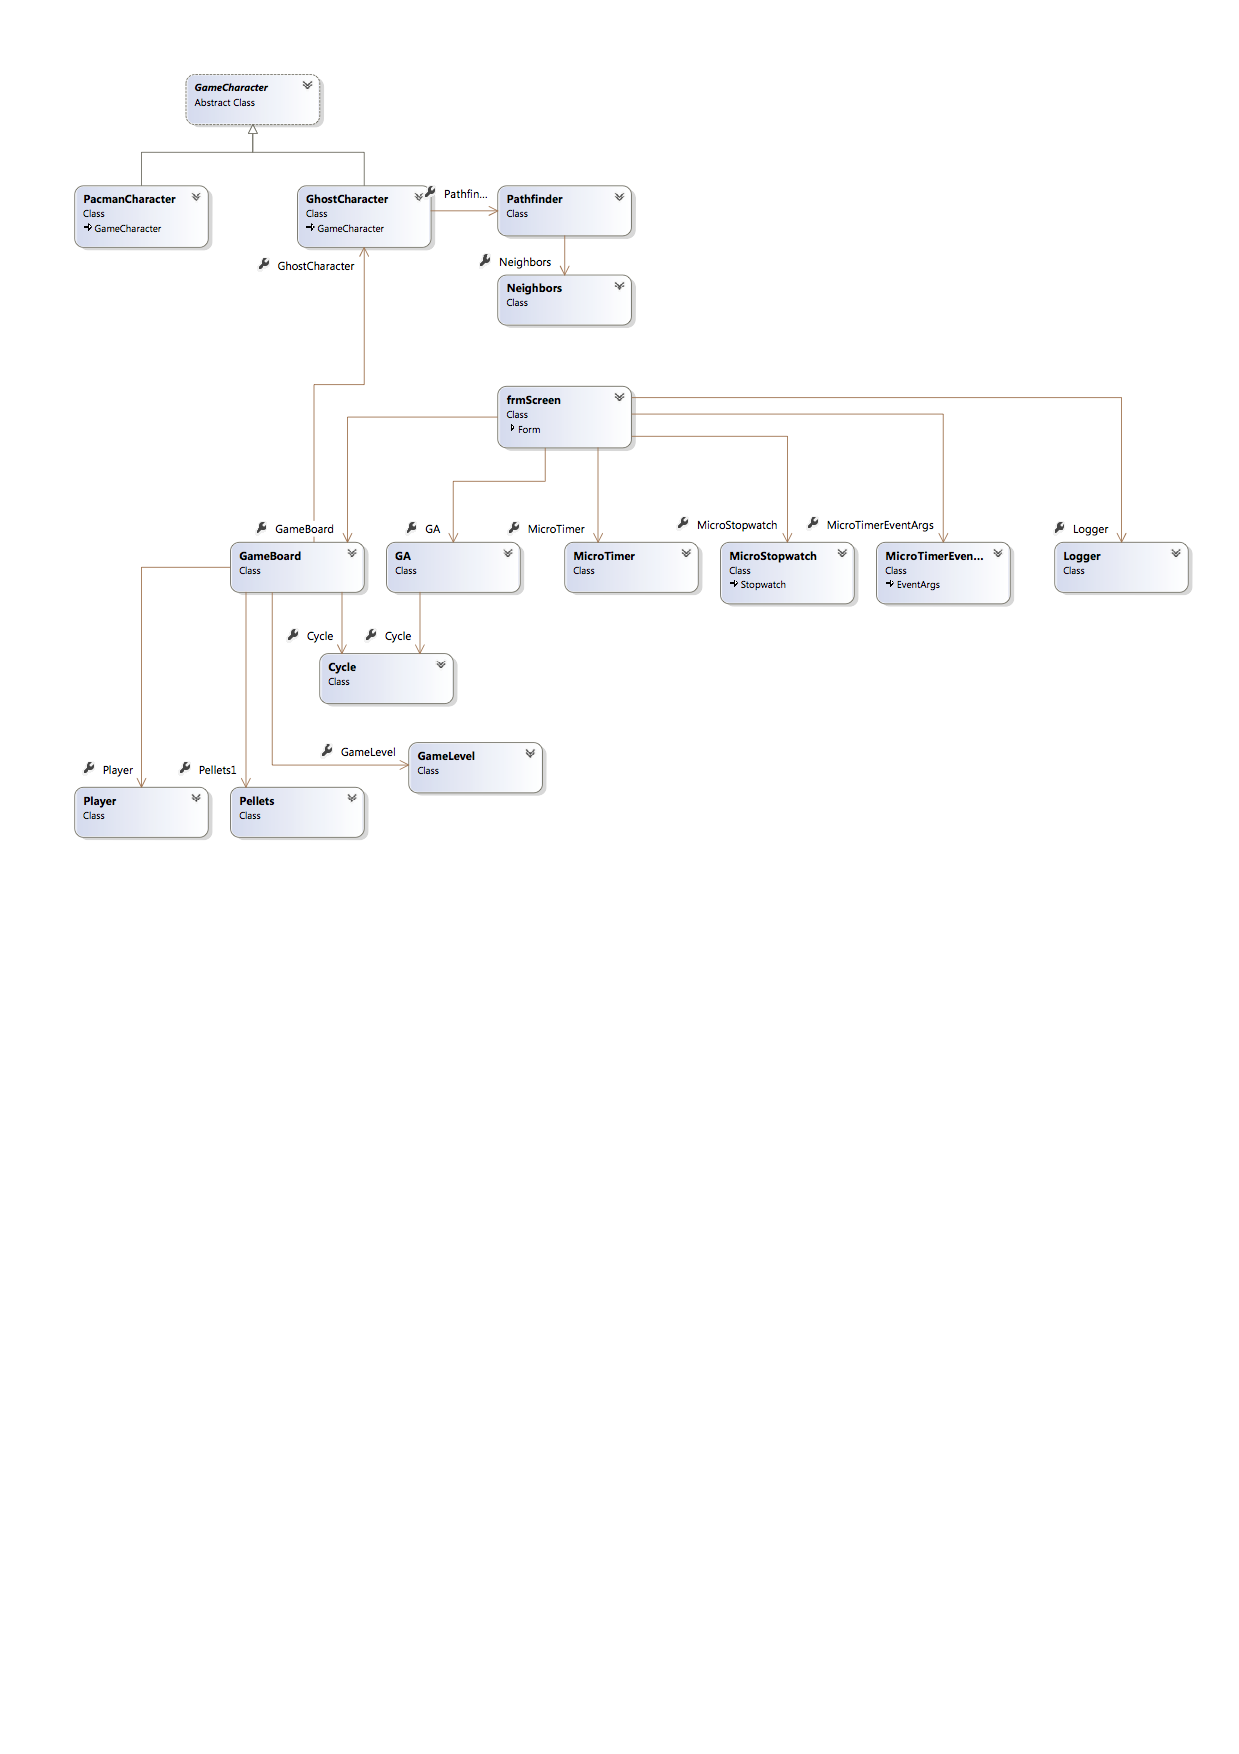
\includegraphics[width=1.00\textwidth]{ClassDiagram.png}
	\caption{Class diagram with inheritance and interfacing between the classes}
	\label{fig:class}
\end{figure}

